\comment{The}{Revoir l'anglais en profondeur, je n'ai pas compris grand chose de cet exemple et la formulation du problème n'est pas présente} goal was to estimate in real-time joint kinematic and muscle activation using a moving horizon estimation (MHE). 
Therefore, muscle driven optimal control problem using a 4DoFs and 18 muscles arm model was built and split into a succession of smaller \comment{one}{smaller models?}.
Thanks to the high similarity between successive problems, a warm-start strategy using previous solutions was implemented. 
Each OCP problems consisted in tracking joint angles \comment{(Eq. 3)}{Utiliser ref}, \comment{minimize muscles controls, for controls regularization, and minimize states, for states regularization. 
At the end, only the first node of each estimation was kept to build the entirely solution.}{Je n'ai rien compris}

A shoulder elevation movement of 8s on 800 frames was generated with co-contraction on the triceps/biceps muscles groups to test estimator. 
A windows size of 7 nodes which allows the estimator to run around 50Hz, four times faster than standard biofeedback (13Hz) was chosen.
Whereas experimental data were generated at 100Hz, only one on two frames was sent to the estimator to correspond with experimental conditions. 
The estimator was able to forecast the movement kinematics (Fig. xx) with a consistent dynamic. 
As expected, the estimated muscles activations are lower than reference motion activation but with similar pattern (Fig. XX). 

\begin{figure*}[t!]
\centering
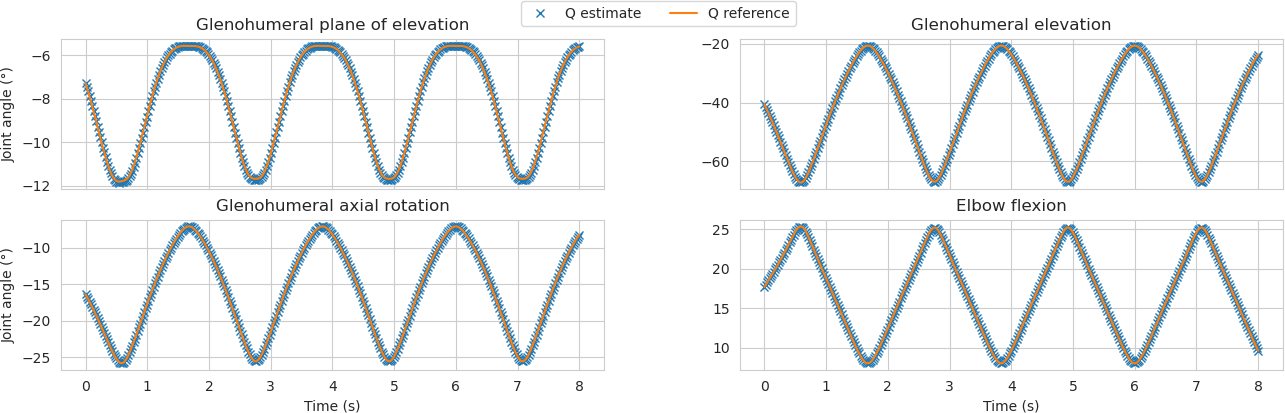
\includegraphics[width=\textwidth]{figures/Articular_angle_MHE.png}\\
\caption{Representation of estimate articlation angles (blue cross) and reference articulation angles (orange line).}
\label{fig:angulare_angle_MHE}
\end{figure*}
\begin{figure*}[t!]
\centering
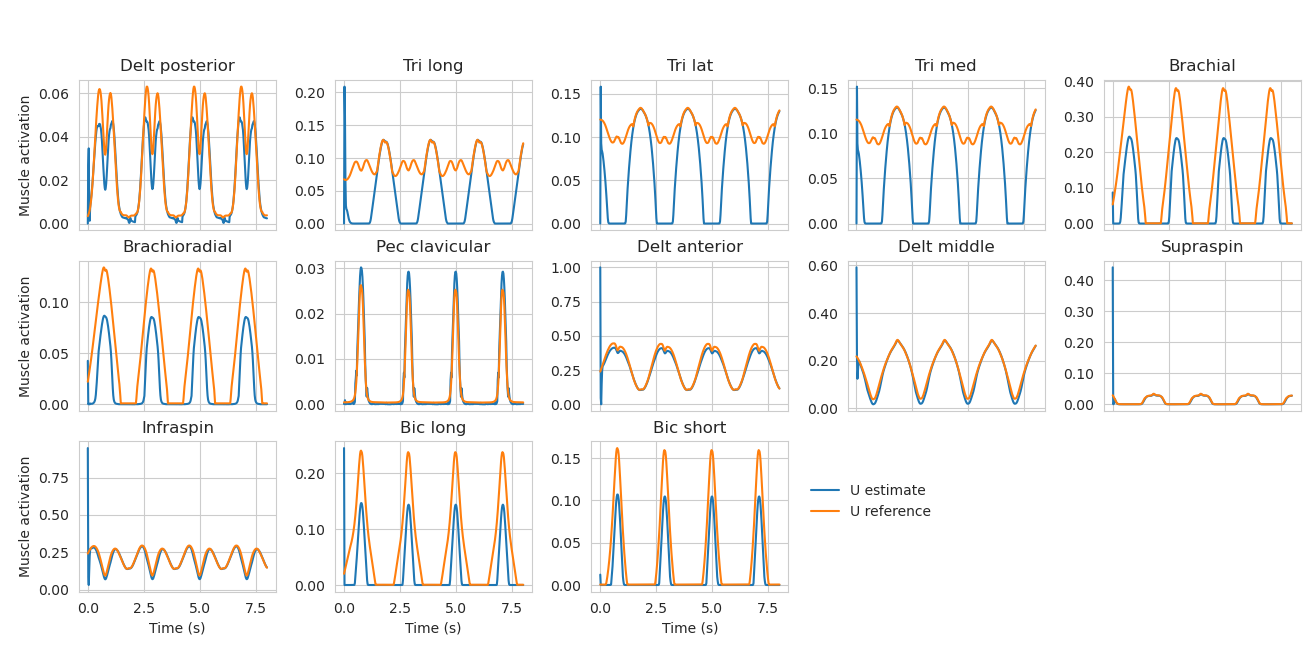
\includegraphics[width=\textwidth]{figures/Muscles_excitations_MHE.png}\\
\caption{Representation of estimate muscles activations (blue) and co-contracted muscles activations(orange) with significative action on motion (activation $>$ 1e-3).}
\label{fig:muscles_excitations_MHE}
\end{figure*}
